\documentclass{beamer}
\usetheme{Madrid}


\title{RFID Sicherheit}
\author{Julian Hoever}
\date{24. Juni 2020}

\begin{document}

\begin{frame}
\titlepage
\end{frame}


\section{Einleitung}
\begin{frame}
\frametitle{Einleitung}


\begin{itemize}
	\item RFID Technik kommt in vielen alltäglichen Anwendungen vor
	\begin{itemize}
		\item Kontaktloses Bezahlen
		\item Personalausweisen
		\item Zeiterfassung mittels RFID Transponder
	\end{itemize}
	\item Alte aber stetig weiterentwickelte Technik
	\item Durch die Funktionsweise und das Alter der Technik ergeben sich einige Sicherheitsprobleme
\end{itemize}

\begin{figure}
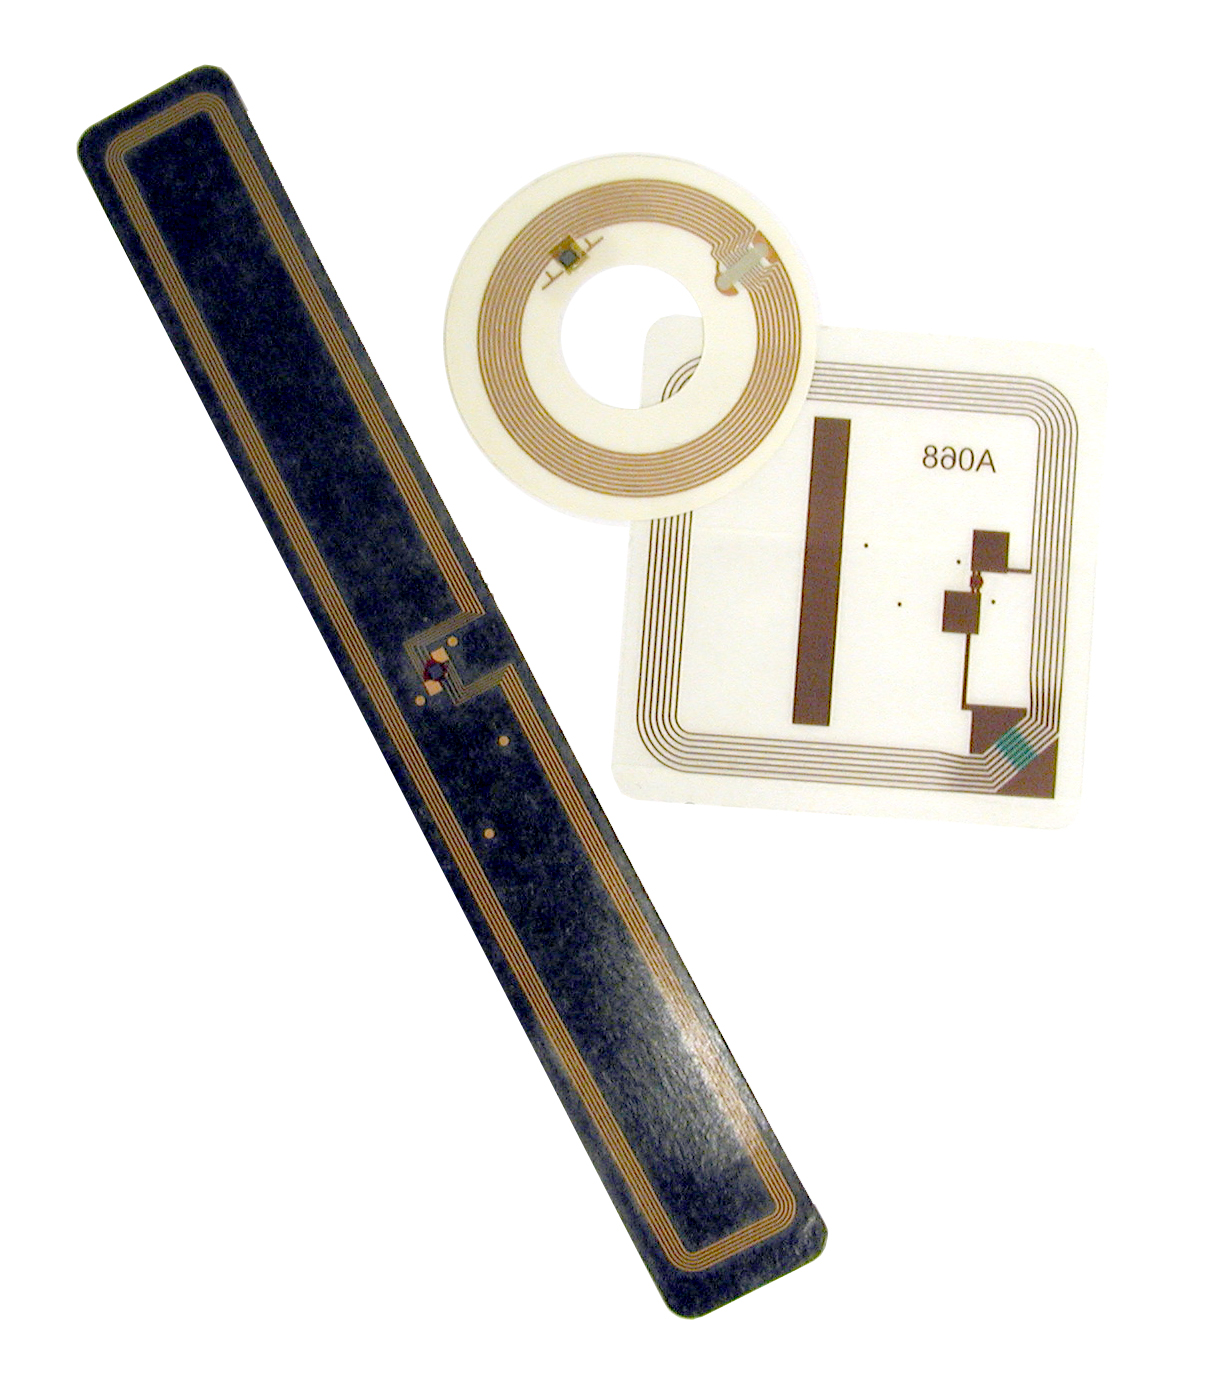
\includegraphics[width=0.2\textwidth]{img/RFID_Tags.jpg}
\caption{Verschiedene RFID Transponder \footnote{https://upload.wikimedia.org/wikipedia/commons/e/e3/RFID\_Tags.jpg}}
\end{figure}
\end{frame}


\section{Grundlagen}
\begin{frame}
\frametitle{Grundlagen}
\begin{itemize}
	\item Lesegerät liest Daten aus einem Transponder
	\item Transponder gibt es in vielen Größen und Formen
	\item Grundlegender Aufbau eines Transponders:
	\begin{itemize}
		\item Spulenförmige Antenne
		\item Schaltkreise zum Senden/Empfangen
		\item Speicher
	\end{itemize}
	
	\item Aktive/Passive Transponder
	\begin{itemize}
		\item Aktiver Transponder $\rightarrow$ eigene Spannungsquelle
		\item Passiver Transponder $\rightarrow$ keine eigene Spannungsquelle
	\end{itemize}
\end{itemize}
\end{frame}


\begin{frame}
\frametitle{Grundlegendes Kommunikationsschema}

\begin{enumerate}
	\item Lesegerät induziert Spannung und Taktfrequenz
	\item Lesegerät sendet Anfrage an Transponder
	\item Transponder übermittelt entsprechende Daten
\end{enumerate}

\begin{figure}
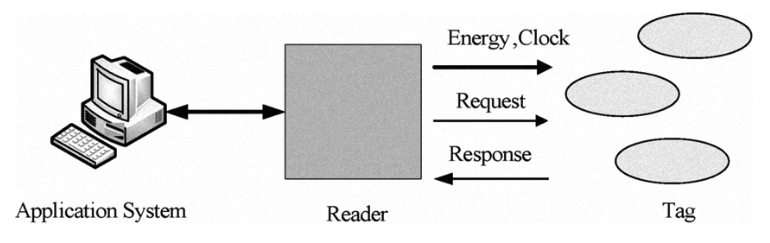
\includegraphics[width=0.7\textwidth]{img/kommunikation.png}
\caption{Kommunikationsschema \footnote{Chih-Yung Chen, Chien-Ping Kuo and Fang-Yuan Chien, "An exploration of RFID information security and privacy"}}
\end{figure}
\end{frame}


\section{Schwachstellen}
\begin{frame}
\frametitle{Schwachstellen}

\begin{itemize}
	\item Fehlende Authentifikation
	\begin{itemize}
		\item Transponder übermittelt Speicherinhalt auf Anfrage
		\item Jedes Lesegerät kann den Transponder lesen
	\end{itemize}
	
	\item Übertragung im Klartext
	\begin{itemize}
		\item Ursprünglich Übertragung im Klartext standardisiert
		\item Übertragung kann abgehört werden
	\end{itemize}
	
	\item Energieversorgung
	\begin{itemize}
		\item Energieversorgung durch das Lesegerät mittels Induktion
		\item Passiver Transponder ist darauf angewiesen
	\end{itemize}
\end{itemize}
\end{frame}


\begin{frame}
\frametitle{Schwachstellen}

\begin{itemize}
	\item Eindeutige Identifikation
	\begin{itemize}
		\item Identifizierung durch Speicherinhalt und Identifikationsnummer
		\item Ermöglicht Tracking
	\end{itemize}
	
	\item Lesegerät kennt Daten nicht
	\begin{itemize}
		\item Daten müssen gelesen und verarbeitet werden
		\item Bedrohung für Softwareinfrastruktur
	\end{itemize}
	
	\item Lesegerät muss Transponder lesen
	\begin{itemize}
		\item Lesegerät kann nicht entscheiden wie relevant ein Transponder ist ohne ihn zu lesen
		\item Lesevorgang belegt Rechenkapazität des Lesegerätes
	\end{itemize}
\end{itemize}
\end{frame}


\section{Angriffe auf Sicherheit und Privatsphäre}
\begin{frame}
\frametitle{Angriffe auf Sicherheit und Privatsphäre}

\begin{itemize}
	\item Folgende Schwachstellen werden genauer betrachtet:
	\begin{itemize}
		\item Fehlende Authentifikation
%		\item Lesegerät kennt Daten nicht
		\item Energieversorgung
	\end{itemize}
\end{itemize}
\end{frame}


\begin{frame}
\frametitle{Fehlende Authentifikation}

\begin{itemize}
	\item Unbefugte können Transponder lesen
	\item Kopieren von Transpondern
	\begin{itemize}
		\item Jedes Lesegerät kann einen Transponder lesen
		\item Gelesene Daten können auf neuen Transponder geschrieben werden
		\item Daten der Kopie sind identisch mit dem Original
		\item Flüchtigen Kontakt mit dem Originaltransponder 
	\end{itemize}
	\item Gefahr für beispielsweise Türsteuerungen
	\item Persönliche Daten könnten aus dem Transponder gelesen werden
\end{itemize}
\end{frame}


\begin{frame}
\frametitle{Sicherheitsmaßnahmen}

\begin{itemize}
	\item Verschiedene Ansätze eine Authentifikation zu implementieren
	\begin{itemize}
		\item Unterscheidung in Sicherheit und Komplexität
	\end{itemize}
	
	\item MIFARE Classic EV1 \footnote{https://www.nxp.com/docs/en/data-sheet/MF1S70YYX\_V1.pdf}
	\begin{itemize}
		\item RFID Transponder mit 13.56 MHz Frequenz
		\item Speicher in Sektoren aufgeteilt
		\item Sektoren unterteilt in 16 Byte Blöcke
		\item Jeder Sektor kann separat ausgelesen werden
		\begin{itemize}
			\item Separate Authentisierung für jeden Sektor
		\end{itemize}
		\item Sector Trailer
		\begin{itemize}
			\item Letzter Block eines Sektors
			\item Schlüssel A, Zugriffsbedingungen, Schlüssel B (optional)
		\end{itemize}
	\end{itemize}
\end{itemize}
\end{frame}


\begin{frame}
\frametitle{Sicherheitsmaßnahmen}

\begin{itemize}
	\item Drei-Phasen-Authentifikation der MIFARE Classic EV1 \footnote{https://www.nxp.com/docs/en/data-sheet/MF1S70YYX\_V1.pdf}
\end{itemize}

\begin{figure}
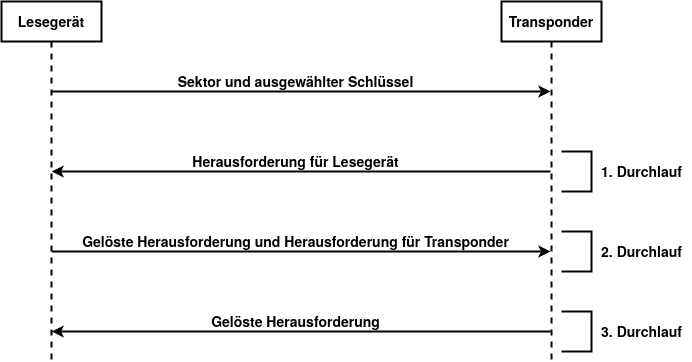
\includegraphics[width=0.8\textwidth]{img/three_pass.png}
\end{figure}
\end{frame}


\begin{frame}
\frametitle{Sicherheitsmaßnahmen}

\begin{itemize}
	\item Rechteverwaltung durch Drei-Phasen-Authentifikation
	\begin{itemize}
		\item Separate Schlüssel für jeden Sektor
		\item Lesegerät kann nur Sektoren lesen für das es den Schlüssel besitzt
	\end{itemize}
	\item Leistungsfähiger Transponder benötigt
	\item Schutz vor Vervielfältigung und unberechtigtem Zugriff
	
	\item Alternatives Authentifikationsverfahren
	\begin{itemize}
		\item Einfaches Passwort
		\item Kommunikationspartner tauchen Passwort zu Beginn aus
		\item Problem: Übertragung im Klartext
	\end{itemize}
\end{itemize}
\end{frame}


\begin{frame}
\frametitle{Durchführbarkeit}

\begin{itemize}
	\item Kopieren und Auslesen sehr leicht durchführbar
	\begin{itemize}
		\item Kurzer Kontakt
		\item Unbeaufsichtigte Brieftasche, Schlüsselbund, etc.
	\end{itemize}
	\item Heutzutage wirkungsvolle Authentifizierungsmaßnahmen
	\item Transponder ohne Authentifizierung sind ein erhebliches Sicherheitsrisiko
	\item Sicherheitsanforderungen hängen von Anwendung ab
\end{itemize}
\end{frame}


\begin{frame}
\frametitle{Energieversorgung}

\begin{itemize}
	\item Denial of Service Angriff
	\begin{itemize}
		\item Transponder wird vor elektrischem Feld abgeschirmt
		\begin{itemize}
			\item[$\Rightarrow$] Faradayscher Käfig
		\end{itemize}
		\item Energieversorgung wird unterbunden 
		\item Lesegerät erkennt den Transponder nicht
	\end{itemize}
	
	\item Problem bei der Warensicherung mittels RFID
\end{itemize}

\begin{figure}
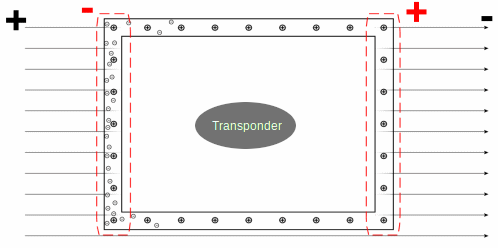
\includegraphics[width=0.5\textwidth]{img/kaefig.png}
\caption{Transponder im Faradayschen Käfig \footnote{https://commons.wikimedia.org/wiki/File:Faraday\_cage.gif\#/media/ Datei:Faraday\_cage.gif}}
\end{figure}
\end{frame}


\begin{frame}
\frametitle{Sicherheitsmaßnahmen}

\begin{itemize}
	\item Transponder sind abhängig von elektrischem Feld
	\item Transponder für das Lesegerät nicht existent
	\item Schwachstelle kann nicht ohne weiteres behoben werden
	\item Zusätzliche Maßnahmen je nach Anwendung:
	\begin{itemize}
		\item Videoüberwachung
		\item Ladendetektiv
		\item ...
	\end{itemize}
\end{itemize}
\end{frame}


\begin{frame}
\frametitle{Durchführbarkeit}

\begin{itemize}
	\item Denial of Service Angriffe auf Transponder sind sehr leicht durchführbar
	\item RFID blockierende Beutel ($\Rightarrow$ Faradayscher Käfig)
	\item Hohes Schadenspotenzial
	\begin{itemize}
		\item z.B. Diebstahlsicherungen im Einzelhandel
	\end{itemize}
\end{itemize}
\end{frame}

\section{Fazit}
\begin{frame}
\frametitle{Fazit}

\begin{itemize}
	\item RFID bietet viele Möglichkeiten
	\begin{itemize}
		\item Kontaktloses Bezahlen, Diebstahlsicherung, Kontaktlose Zugangskontrollen, etc...
	\end{itemize}
	\item Schwachstellen beachten
	\item Sicherheit an die jeweiligen Anforderungen anpassen
	\item Privatsphäre der Nutzer beachten
\end{itemize}
\end{frame}


\end{document}